\section{Критерий устойчивости уравнений с постоянными коэффициентами}

	В данном разделе мы будем рассматривать критерий Рауса-Гурвица об устойчивости линейных уравнений $n$-го порядка с постоянными коэффициентами. Согласно условиям, решение линейного уравнения с постоянными коэффициентами является устойчивым, если вещественные части корней соответствующего характеристического полинома отрицательны. Необходимым условием является положительность коэффициентов уравнения.

	Рассматривать будем линейное уравнение следующего вида:
	\[ a_0 y^{(n)} + a_1 y^{(n-1)} + \cdots + a_{n-1} y' + a_n y = 0, ~ a_i \in \mathbb{R}, ~ a_i > 0 ~ \forall i = \overline{0, n}. \]
	Соответствующий характеристический полином имеет следующий вид:
	\[ P\pares{\lambda} = a_0 \lambda^n + a_1 \lambda^{n-1} + \cdots + a_{n-1} \lambda + a_n. \]
	Решение является асимптотически устойчивым, если вещественные части корней уравнения $P\pares{\lambda} = 0$ отрицательны. Для определения отрицательности корней можно воспользоваться критерием Рауса-Гурвица. Согласно критерию, необходимо, чтобы все главные миноры матрицы Гурвица были положительными. Матрица Гурвица строится по следующим правилам:
	\begin{itemize}
		\item На главной диагонали располагаются коэффициенты характеристического уравнения, начиная с $a_1$;
		\item В столбцах коэффициенты характеристического уравнения располагаются по убыванию;
		\item В ячейках, где индекс коэффициента ниже минимального или выше максимального ставятся нули.
	\end{itemize}
	По заданным правилам, матрица Гурвица выглядит следующим образом:
	\[ G = \begin{pmatrix}
		a_1 & a_3 & a_5 & \cdots & 0 & 0 \\
		a_0 & a_2 & a_4 & \cdots & 0 & 0 \\
		0 & a_1 & a_3 & \cdots & 0 & 0 \\
		\vdots & \vdots & \vdots & \ddots & \vdots & \vdots \\
		0 & 0 & 0 & \cdots & a_{n-1} & 0 \\
		0 & 0 & 0 & \cdots & a_{n-2} & a_n \\
	\end{pmatrix}. \]

	\subsection{Примеры}

		Рассмотрим пример. Для следующего уравнения определить, при каких значениях параметров $a, b$ решение является асимптотически устойчивым:
		\[ y^{IV} + 2y''' + a y'' - by' + 3y = 0. \]
		Согласно необходимому условию, коэффициенты уравнения должны быть положительны. Тогда, первое необходимое условие устойчивости: $a > 0, b < 0$. Построим матрицу Гурвица:
		\[ G = \begin{pmatrix}
			2 & -b & 0 & 0 \\
			1 & a & 3 & 0 \\
			0 & 2 & -b & 0 \\
			0 & 1 & a & 3
		\end{pmatrix}. \]
		Найдем главные миноры:
		\[ M_1 = \begin{vmatrix} 2 \end{vmatrix} = 2 > 0, ~ M_2 = \begin{vmatrix} 2 & -b \\ 1 & a \end{vmatrix} = 2a + b > 0, \]
		\[ M_3 = \begin{vmatrix}  
			2 & -b & 0 \\
			1 & a & 3 \\
			0 & 2 & -b \\
		\end{vmatrix} = 2 \begin{vmatrix} a & 3 \\ 2 & -b \end{vmatrix} - \begin{vmatrix} -b & 0 \\ 2 & -b \end{vmatrix} = -2ab - 12 - b^2 > 0, \]
		\[ M_4 = \begin{vmatrix}
			2 & -b & 0 & 0 \\
			1 & a & 3 & 0 \\
			0 & 2 & -b & 0 \\
			0 & 1 & a & 3
		\end{vmatrix} = 3M_3 > 0. \]
		Согласно критерию, необходимо, чтобы все миноры были положительны. Последний минор зависит от предпоследнего, соответственно, если $M_3 > 0$, то и $M_4 > 0$. Выпишем систему неравенств:
		\[ \syst{
			&a > 0, ~ b < 0, \\
			& 2a + b > 0, \\
			&b^2 + 2ab + 12 < 0.
		} \implies \syst{
			&a > 0, ~ b < 0, \\
			&b > -2a, \\
			&b^2 + 2ab + 12 < 0.
		} \]
		Условие $b > -2a$ не противоречит условию $b < 0$ при $a > 0$, и является усиляющим. Из последнего условия найдем ограничения для $b$:
		\[ -a - \sqrt{a^2 - 12} < b < -a + \sqrt{a^2 - 12}. \]
		Для того, чтобы $b$ было вещественным, необходимо, чтобы $a \ge \sqrt{12}$ или $a \le -\sqrt{12}$ (что противоречит условию $a > 0$). Условие $a \ge \sqrt{12}$ является усиляющим. При $a \ge \sqrt{12}$, $a > \sqrt{a^2 - 12}$. Также $-2a < -a - \sqrt{a^2 - 12} < -a + \sqrt{a^2 - 12}$, что также является усиляющим условием. Объединим все сильные условия. Таким образом, решение исходной задачи является асимптотически устойчивым при:
		\[ \syst{&a \ge \sqrt{12}, \\ &-a - \sqrt{a^2 - 12} < b < -a + \sqrt{a^2 - 12},} \]
		или, что то же:
		\[ \syst{&a \ge 2\sqrt{3}, \\ &b^2 + 2ab + 12 < 0.} \]
		На плоскости $a, b$ соответствующая область выглядит таким образом:
		\begin{figure}[H]
			\centering
			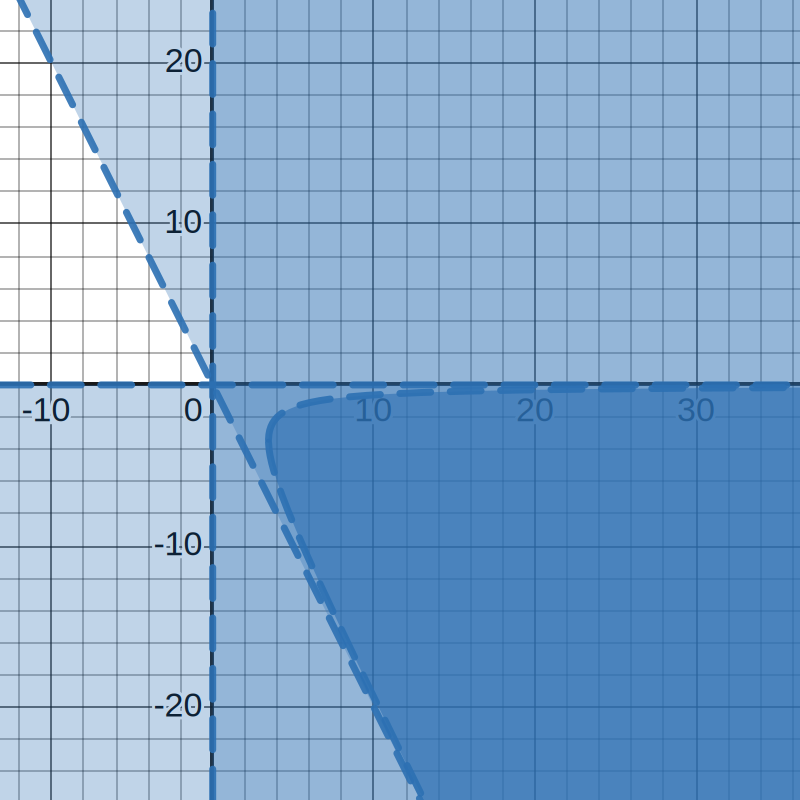
\includegraphics[width=0.5\textwidth]{additional/Stability/ranges.pdf}
			\caption{Область параметров $a, b$}
		\end{figure}
